\PassOptionsToPackage{cmyk,table}{xcolor}
\documentclass[conference,flushend]{iaria}
\pdfoutput=1 % pdflatex hint for arxiv.org (within first 5 lines)

% en-US  = [english]/[american]/[USenglish] <DEFAULT>
\usepackage[babel=true,english=american]{csquotes}
\usepackage[english]{babel} % en-US
% IARIA requires uppercase TABLE, and babel intervenes in the tablename
\addto\captionsenglish{\renewcommand\tablename{TABLE}}
% en-UK  =           [british] /[UKenglish] <OXFORD>
%\usepackage[babel=true,english=british]{csquotes}
%\usepackage[british]{babel} % en-UK
%% IARIA requires uppercase TABLE, and babel intervenes in the tablename
%\addto\captionsbritish{\renewcommand\tablename{TABLE}}

% Allows to hyphenate a word that contains a dash:
% https://stackoverflow.com/questions/2193307/how-do-i-get-latex-to-hyphenate-a-word-that-contains-a-dash
\usepackage[shortcuts]{extdash} % Use \-/ for a breakable dash that does not prevent the remainer of the word to be hyphenated

\usepackage[alwaysadjust]{paralist}
\usepackage[caption=false,font=footnotesize]{subfig}

% Class iaria.cls loads biblatex / biber with predefined options
\addbibresource{embedded.bib}
\addbibresource{cpn_all_all.bib}

\usepackage[
babel=true, % Enable language-specific kerning. Take language-settings from the languge of the current document (see Section 6 of microtype.pdf)
expansion=alltext,
protrusion=alltext-nott, % Ensure that at listings, there is no change at the margin of the listing
nopatch=eqnum, % fix unable to apply patch eqnum
final % Always enable microtype, even if in draft mode. This helps finding bad boxes quickly.
% In the standard configuration, this template is always in the final mode, so this option only makes a difference if "pros" use the draft mode
]{microtype}


%
% packages added by K.Böhm (not included in the template)
%
%\usepackage{svg} %does not work under Windows due to the need of external tools

% --- end of own packages included ----
\begin{filecontents}[overwrite]{embedded.bib}
@online{ieee2015howto,
    author = {Michael Shell},
    title = {How to Use the {IEEEtran} \LaTeX\ Class},
    url = {http://mirrors.ctan.org/macros/latex/contrib/IEEEtran/IEEEtran_HOWTO.pdf},
    year = {2015}
}
@online{ieee2018formattingrules,
    author = {{IEEE}},
    title = {Conference Template and Formatting Specifications},
    url = {https://www.ieee.org/content/dam/ieee-org/ieee/web/org/conferences/Conference-template-A4.doc},
    year = {2018}
}
@online{iaria2014formattingrules,
    author = {{IARIA}},
    title = {Formatting Rules},
    url = {http://www.iaria.org/formatting.doc},
    year = {2014}
}
@online{iaria2009editorialrules,
    _author = {Cosmin Dini},
    author = {{IARIA}},
    title = {Editorial Rules},
    url = {https://www.iaria.org/editorialrules.html},
    year = {2009}
}
@online{languagetool,
    author = {{LanguageTooler GmbH}},
    title  = {{LangueTool}},
    url    = {https://languagetool.org/overleaf}
}
@online{overleaf,
    author = {{Digital Science UK Limited}},
    title  = {{Overleaf}},
    url    = {https://www.overleaf.com}
}
\end{filecontents}

\usepackage{fontawesome} % i.a., \faWarning{}
\usepackage{relsize}     % i.a., \textsmaller{...}
\usepackage{lipsum}      % for blindtext

% ======================================================================

% https://www.silbentrennung24.de/
% https://www.hyphenation24.com/
\hyphenation{block-chain block-chains Ethe-re-um}

% Capitalization: https://capitalizemytitle.com/style/Chicago/
\title{The \textsmaller{IARIA} Example of its \textsmaller{CTAN} Package and \LaTeX{} Class}

\author{
    \IEEEauthorblockN{Karsten Böhm\,\orcidlink{0000-0002-2950-7433}}
    \IEEEauthorblockA{%
        FH Kufstein Tirol - University of Applied Sciences\\
        Kufstein, Austria\\
        % Diferring from IEEE ("Email"), IARIA requires "e-mail":
        e-mail: \texttt{karsten.boehm@fh-kufstein.ac.at}
        % Multiple authors and their e-mail addresses:
        %e-mail: {\tt$\lbrace$j.smith\,|\,c.neumann$\rbrace$@oth-aw.de}
    }
}

\begin{document}

\maketitle

\begin{abstract}
This paper demonstrates an example of a paper, based on the \texttt{iaria} \LaTeX{} class.
The example is intended for beginners, e.\,g., undergraduate students.
It contains a basic outline template and usually fills it with dummy text.
Graphic exclamation marks highlight important remarks.
%
\{\,\faWarning{} For beginners:
Do NOT remove the abstract, this section is mandatory.
Do NOT use special characters, symbols, or math in your title or abstract.
Do NOT use cites in your abstract.\}
\end{abstract}

% A list of IEEE Computer Society appoved keywords can be obtained at
% http://www.computer.org/mc/keywords/keywords.htm
\begin{IEEEkeywords}
    % Diferring from IEEE, IARIA requires also the keywords in Bold and Italic (and lower case):
    template; lorem ipsum.
\end{IEEEkeywords}

\section{Introduction}

The \textsmaller{IARIA} formatting is based on \textsmaller{IEEE} style.
The unofficial \textsmaller{IARIA} \LaTeX\ class is based on \textsmaller{IEEE}tran class \cite{ieee2015howto}.
The \textsmaller{IARIA} formatting rules \cite{iaria2014formattingrules} are adopted from the \textsmaller{IEEE} template and formatting specifications \cite{ieee2018formattingrules}.
In addition, be aware of the supplementary \textsmaller{IARIA} editorial rules \cite{iaria2009editorialrules} \faWarning{} that provide a beginner-friendly set of further advices.
It is recommended to use a grammar tool, e.\,g., the LanguageTool \cite{languagetool} browser plugin in combination with Overleaf \cite{overleaf}.

\lipsum[22]

\{\faWarning{} \textsmaller{IARIA} editorial rules: Introduction must end with a paragraph describing the structure of the paper!\}
The remainder of the paper is organized as follows: In Section~II, …

\section{Related work \textbar{} Methods}
\lipsum[23]

\section{Results}
\lipsum[24]

\section{Discussion \textbar{} Evalution}
This is the discussion with a first sentence and a figure to be included here.

\begin{figure}[ht]
	\centering
	\includegraphics[width=0.9\linewidth]{D:/Bilder/Camera/2025-01-04_Laufen-Rosenheim/IMG20250104163930}
	\caption[Sample image]{This is just a sample image with a long description in the label}
	\label{fig:img_sample1}
\end{figure}

we also check whether we can properly include SVG graphics as this is one of our mayjor formats that we will use here


\begin{figure}[htbp]
	\centering
	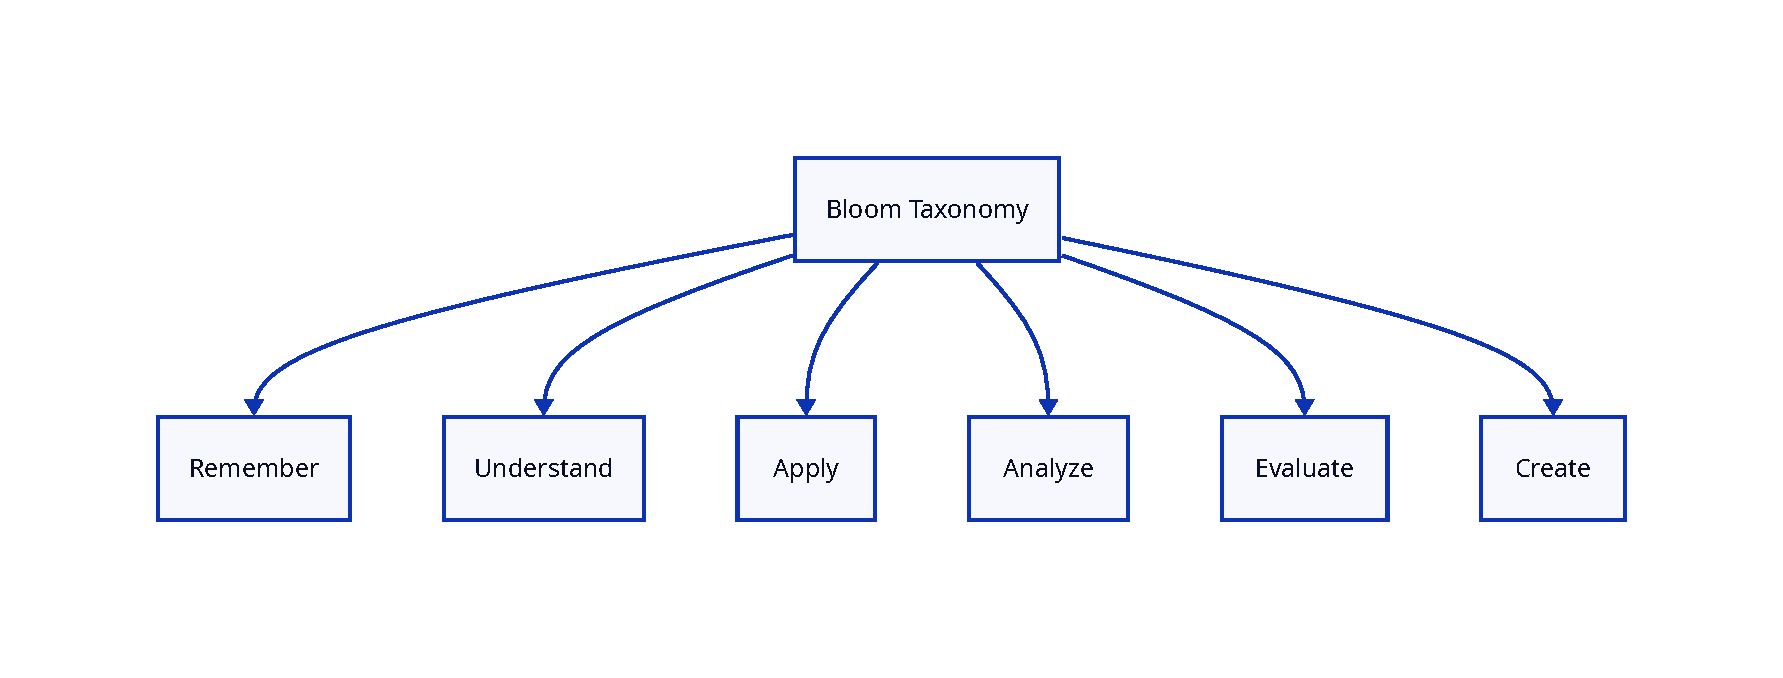
\includegraphics[width=1.0\linewidth]{img/bloom.pdf}
	\caption{svg image this is a sample for an SVG}
\end{figure}

\lipsum[25]

\section{Conclusion and Future Work}
\{\faWarning{} \textsmaller{IARIA} editorial rules: Last section must be \textquote{Conclusion and Future Work}!\}
\lipsum[26]

\{\,\faWarning{} For beginners: you must not leave the bibliography blank. Add appropriate references to your related work.\}
%
%\vspace{\baselineskip}
A selection of previous  \textsmaller{IARIA} publications of the CyberLytics lab
%
%
%% INSTRUCTION: Remove the irrelevant ones and cite
%% the ones that are actually related on technological
%% level or that address the same domain.
%% This listing is just as a stimulus:
\cite{%
LeNe24goalHijackingLLMs,%
LeNe24vocattllm,%
PANP23seccloudfogai,%
StNe23foodfresh}
%
%
are included as reference and further example.

% ======== References =========
\begingroup
\sloppy
\printbibliography
\endgroup 

\end{document}
